\chapter*{Commentary}
\addcontentsline{toc}{chapter}{Commentary}

Data management is a broad field that encompasses various aspects of handling data, such as modeling, storage, querying, and evolution. For years, the focus of data management research has been on relational data, which is structured in tables with fixed schemas~\citep{DBLP:persons/Codd71a}. In the early 2000s, the rise of \acrshort{nosql} databases~\citep{PolyglotPersistance} introduced new data models and formats, such as document, graph, key-value, and columnar.

These models offer distinct advantages for certain types of applications and workloads, making them popular choices for handling unstructured, highly dynamic, or large-scale data (all of which are common characteristics of modern data). However, this diversity of data models comes with its own set of challenges. Whereas migration from one relational database to another is relatively straightforward, moving data between databases that use different data models can be complex and error-prone. Generally, the \acrshort{nosql} world lacks unified theoretical foundations, common standards, and tools that would leverage them for managing data across various models~\citep{CSUR-Jiaheng}.

In real-world scenarios, these complex use cases involving multiple data models and databases are becoming increasingly common. Such data is often referred to as \term{multi-model data} (in contrast to the traditional approach of \term{single-model data}). \Cref{fig:mm_data} shows an example of multi-model data, based on a subset of the \emph{Yelp Academic Dataset}\footnotei{\url{https://www.kaggle.com/datasets/yelp-dataset/yelp-dataset}}{.} The original dataset consists of \acrshort{json} collections, but to optimize query performance, we might decide to store \code{user} in a relational database, \code{business} in a document database, \code{FRIEND} in a graph database, and \code{review} in a columnar database. Crucially, the data in these models is still connected via the same identifiers, because in some use cases, we need to combine data from different models in a single query.

\begin{figure}[ht]
    \centering
    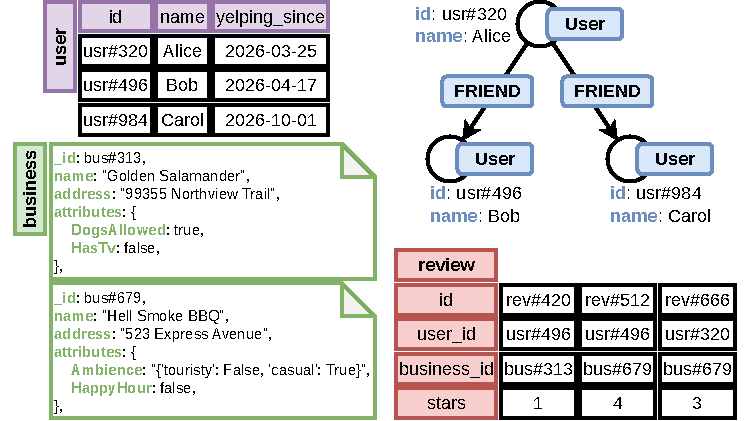
\includegraphics[width=\textwidth]{img/commentary-mm_data.drawio.pdf}
    \caption{Example of multi-model data, based on a subset of the \emph{Yelp Academic Dataset}, organized to different data models---relational (purple), document (green), graph (blue), and columnar (red).}
    \label{fig:mm_data}
\end{figure}

\todo{
- jedna DB nemusí stačit (i když je MM), můžeme chtít jiné škálování

- redundance?
}

\subsubsection{Outline}

The rest of this chapter provides a high-level overview of the whole thesis. It includes the vision for our research, asks the open questions we want to address, and describes the overall approach we take to answer them. \paperRef{vldb_2024} contains a more detailed description of the vision. \paperRef{cikm_2022} introduces the main concepts of \term{MM-cat}, a framework for multi-model data management that we use as the basis for our research.

\paperRef{edbt_2024} defines the basics of evolution propagation to queries, while \paperRef{rcis_2025} describes the next step of this process, which is the ability to choose between different propagation strategies. \paperRef{vldb_2025_fdephunter} then focuses on the discovery of functional dependencies, which are crucial for making informed decisions about query propagation. \paperRef{dke_2026} compares various index selection methods, which are an important part of self-adaptation, while \paperRef{edbt_2026} describes a holistic approach to self-adaptation.

The next two papers---\paperRef{enase_2025} and \paperRef{edbt_2025}---improve our ability to test the proposed framework by providing tools for generating synthetic multi-model data and queries. Finally, \paperRef{vldb_2025_dortdb} goes beyond our approach by exploring a different way of multi-model data querying.
